\begin{frame}
\begin{center}{\large Why use version control}\end{center}

  \begin{itemize}
    \item Manage your source code (SCM)
    \item Keep a trace of every modification
    \item Come back to any previous state
    \item Collaborate
  \end{itemize}

\end{frame}

\begin{frame}
\begin{center}{\large How does it work}\end{center}
\end{frame}

\begin{frame}
\begin{center}{\large cpold}\end{center}
  horgix@avalon $~$/cpold\$ ls \\
  file                    file.OK             file.old.old \\
  file.2013-08-12         file.old            file.old.test \\
  file.2013-11-15.ok      file.OLD            file.horgix \\
  file.to-check           file.backup         file.old.not-working \\
  horgix@avalon $~$/cpold\$
\end{frame}
\begin{frame}
\begin{center}{\large Local}\end{center}

  \begin{center}
    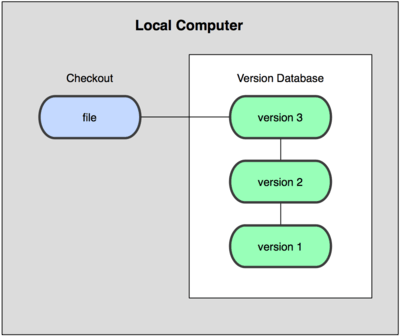
\includegraphics[scale=0.5]{img/local.png}
  \end{center}

\end{frame}
\begin{frame}
\begin{center}{\large Vocabulary}\end{center}

  \begin{itemize}
    \item commit
    \item push
    \item pull
    \item revert
    \item merge
  \end{itemize}

\end{frame}
\begin{frame}
\begin{center}{\large Centralized}\end{center}

  \begin{center}
    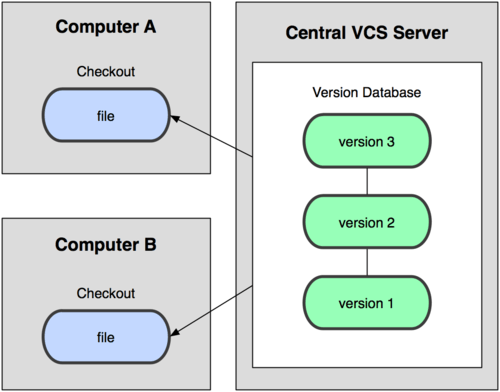
\includegraphics[scale=0.5]{img/centralized.png}
  \end{center}

\end{frame}
\begin{frame}
\begin{center}{\large Distributed}\end{center}

  \begin{center}
    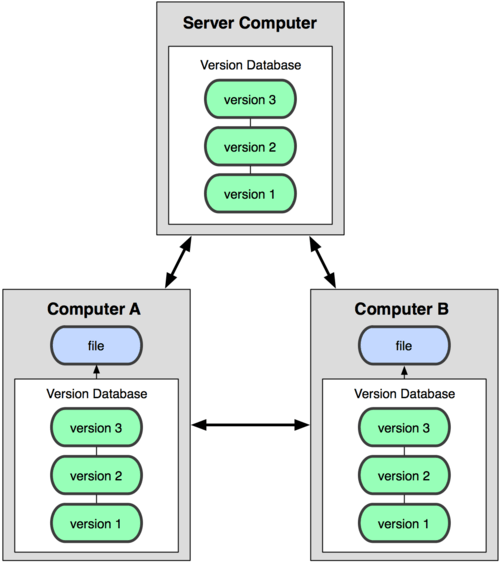
\includegraphics[scale=0.4]{img/distributed.png}
  \end{center}

\end{frame}
\begin{frame}
\begin{center}{\large Some Version Control Systems}\end{center}

  \begin{itemize}
    \item Git
    \item Subversion (SVN)
    \item Mercurial
    \item GNU Bazaar
    \item CVS
    \item Perforce
  \end{itemize}

\end{frame}
\begin{frame}
\begin{center}{\large Git}\end{center}
\end{frame}

\begin{frame}
\begin{center}{\large "Git, c'est le système de rendu d'Epita"}\end{center}

  \begin{itemize}
    \item Google (https://github.com/google)
    \item Facebook (https://github.com/facebook)
    \item Microsoft (http://aspnetwebstack.codeplex.com/)
    \item Twitter (https://github.com/twitter)
    \item Perl (http://perl5.git.perl.org/perl.git)
    \item Android (https://android-review.googlesource.com)
    \item Git (https://git.kernel.org/cgit/git/git.git/)
    \item ...
  \end{itemize}

  G(ot) it ?

\end{frame}
\begin{frame}
\begin{center}{\large Theory}\end{center}
  \begin{center}
  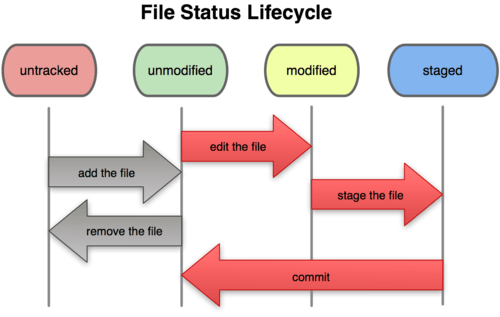
\includegraphics[scale=0.5]{img/lifecycle.png}
\end{center}
\end{frame}
\begin{frame}

\begin{center}{\large Practice}\end{center}

  \begin{itemize}
    \item clone

    \item add

    \item commit

    \item push

    \item pull

    \item conflicts
  \end{itemize}
\end{frame}
\begin{frame}
\begin{center}{\large Good behaviors}\end{center}

  "Commit early, commit often"

  Only commit compiling code.

  Use explicit commit messages.

  Don't add :
  \begin{itemize}
    \item Binaries (.exe, .o, .out, .pdf, ...)
    \item System files (Thumbs.db, ...)
    \item Useless files (git is not a file sharing system)
  \end{itemize}

\end{frame}
\begin{frame}
\begin{center}{\large Where can I host my git repository}\end{center}

  \#\#\# GitHub - https://github.com/

  \begin{itemize}
    \item 5M users
    \item Unlimited contributors
    \item Web pages hosting (GitHub Pages)
  \end{itemize}

  \#\#\# Bitbucket - https://bitbucket.org/

  \begin{itemize}
    \item 1M users
    \item Unlimited free repositories
    \item External authentication (Facebook, OpenID, Google)à
    \item Also supports SVN and Mercurial
  \end{itemize}

\end{frame}
\begin{frame}
\begin{center}{\large Links}\end{center}

  \begin{itemize}
    \item http://git-scm.com/
    \item git.acu.epita.fr
  \end{itemize}

\end{frame}
